\section{Computational performance}\label{sec:performance}

This section reports the measured Track~C benchmark for the four
estimators marked C in Table~\ref{tab:decathlon}: high-dimensional
fixed effects (\code{sp.fast.feols}), Callaway--Sant'Anna staggered
DiD (\code{sp.callaway\_santanna}), classical synthetic control
(\code{sp.synth(method="classic")}), and double machine learning
(\code{sp.dml(model="plr")}). The goal is not to declare universal
speed superiority over the reference implementations. It is to
certify that the unified \proglang{Python}/\pkg{NumPy}/\pkg{Numba} stack is fast enough
for routine applied work, to identify where the \proglang{R}
reference remains faster, and to make the performance tradeoffs
reproducible from the source tree.

\subsection{Benchmark protocol}

The benchmark harness lives under \code{tests/perf/}. Each module has
a \proglang{Python} script and a companion \proglang{R} script that
construct identical seed-fixed synthetic data-generating processes
and record median wall-clock time after one warmup iteration. The
three econometric rows use their canonical \proglang{R} packages; the DML
row uses \pkg{DoubleML} Python so language-runtime and \pkg{R6} dispatch
do not dominate a cheap-linear-learner comparison. All rows were
measured on one machine (Apple Silicon arm64, 8 physical cores, 24~GB
unified memory, macOS~26), with \statspai{} 1.30.1 on the \proglang{Python}
side, after the 1-minute load average had stayed below 1.5 for five
minutes. The \proglang{Python}-side result files record the \statspai{}
version and source commit and the load at the start of each module
(1.35 to 1.67 on eight cores); the reference-side files record the
\proglang{R} and reference-package versions (\pkg{fixest}~0.14.0,
\pkg{did}~2.3.0, \pkg{Synth}~1.1.10), so a timing can be tied to the
release and conditions it describes.
The full per-repetition JSON files are stored under
\code{tests/perf/results/}; \code{tests/perf/compare\_perf.py}
regenerates Table~\ref{tab:track-c-perf} and
Figure~\ref{fig:track-c-loglog}.

All Track-C timings in this paper are CPU timings, because the
reproducibility target is hardware that applied users and reviewers can
obtain without a dedicated accelerator. \statspai{} exposes
accelerator-ready paths for selected workloads (PyTorch CUDA/MPS for
the neural-causal estimators, a JAX backend for the HDFE residualizer,
and \code{sp.fast.feols\_jax} with a \code{jax.vmap}-batched bootstrap
kernel; Section~\ref{sec:perfbackbone}), but those paths do not
support the headline table: GPU acceleration is a backend contract to
be benchmarked on separate hardware, not evidence for a universal speed
claim over \proglang{Stata} or \proglang{R}, whose ecosystems expose
different acceleration models. The experimental Rayon-parallel Rust
kernel and the \code{sp.iv(absorb=...)} HDFE path are likewise excluded
because the submitted build remains reproducible without a compiled
extension.

% Table 13 floats to the top of the following page and used to land
% inside this list, splitting the DML item so that the page opened
% with the fragment "10,000 compares sp.dml(...)". Keep the four
% design descriptions on one page.
\Needspace*{17\baselineskip}
\begin{description}[leftmargin=1.25em,itemsep=0.2em]
\item[HDFE.] A deterministic gravity-style panel with two fixed-effect
factors (firm and year) and $N \in \{10^4,10^5,10^6\}$ rows compares
\code{sp.fast.feols} with \pkg{fixest::feols}~\citep{berge2018efficient}.
\item[CS-DiD.] A balanced staggered-adoption panel with
$N_{\mathrm{units}} \in \{1{,}000,5{,}000,25{,}000\}$ and five time
periods compares \code{sp.callaway\_santanna} with
\pkg{did::att\_gt} plus \pkg{did::aggte}.
\item[SCM.] A two-factor, 30-period synthetic-control panel with
$n_{\mathrm{donors}} \in \{20,50,100\}$ compares
\code{sp.synth(method="classic")} with \pkg{Synth::synth}.
\item[DML.] A partially-linear DML design with linear nuisance learners
and $N = 1{,}000$, 5{,}000, or 10{,}000 compares
\code{sp.dml(model="plr")} with \pkg{DoubleML} Python's PLR estimator.
Both construct their public workflow with the same
\pkg{scikit-learn} linear learners and five folds inside the timed call.
The design isolates wrapper and cross-fitting overhead rather than
benchmarking random-forest training.
\end{description}

\subsection{Measured performance results}

Table~\ref{tab:track-c-perf} reports the largest-size row from each
benchmark module, and Figure~\ref{fig:track-c-loglog} reports the
scaling curve over all measured sizes.

% AUTO-GENERATED by tests/perf/compare_perf.py
\begin{table}[t]
\centering
\begingroup
\footnotesize
\setlength{\tabcolsep}{2pt}
\begin{tabular}{@{}p{0.10\linewidth}p{0.20\linewidth}p{0.13\linewidth}r r r p{0.14\linewidth}@{}}
\toprule
Module & Estimator & Reference & Max. $N$ & sp & Ref. & Faster path \\
\midrule
\code{01\_hdfe} & HDFE 2-way FE & \pkg{fixest} & 1{,}000{,}000 & 0.120 & 0.049 & R $\mathbf{2.5\times}$ \\
\code{02\_csdid} & CS-DiD simple ATT & \pkg{did} & 125{,}000 & 0.027 & 0.175 & sp $\mathbf{6.5\times}$ \\
\code{03\_scm} & Classical SCM & \pkg{Synth} & 100 & 7.476 & 1.871 & R $\mathbf{4.0\times}$ \\
\code{04\_dml} & DML PLR (lin. learners) & \pkg{DoubleML} Python & 10{,}000 & 0.008 & 0.009 & tie $1.14\times$ \\
\bottomrule
\end{tabular}
\endgroup
\caption{Track C measured performance on Apple Silicon arm64 / 8 cores / 24~GB, \statspai{} 1.30.1. Times are median seconds at the largest sample size, across 3 or 5 repetitions after one warmup, using seed-fixed DGPs. Bold denotes a gap of at least $1.5\times$. The DML row uses \pkg{DoubleML} Python with the same linear learners, five folds, and public-workflow construction cost. The Callaway--Sant'Anna row uses a homogeneous-effect DGP favourable to the vectorised group-time loop.}
\label{tab:track-c-perf}
\end{table}


\begin{figure}[t]
\centering
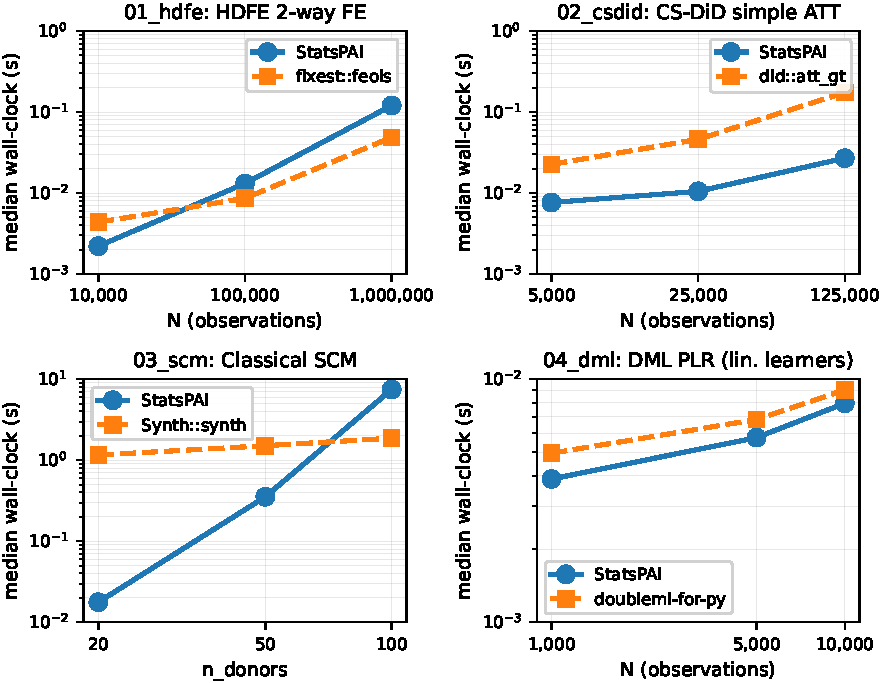
\includegraphics[width=\textwidth]{figures/track_c_loglog.pdf}
\caption{Log-log scaling of \statspai{} versus the declared reference
for the four Track-C benchmarks. The harness
runs both implementations on identical seed-fixed DGPs; points are
median wall-clock seconds across 3 or 5 reps after a warmup. Hardware:
Apple Silicon arm64 / 8 cores / 24~GB / macOS~26. The figure is
regenerated by \code{tests/perf/compare\_perf.py} on every benchmark
run.}
\label{fig:track-c-loglog}
\end{figure}

\paragraph{Reading the scaling figure.}
On the log-log axes of Figure~\ref{fig:track-c-loglog}, a roughly
constant vertical offset between two parallel lines is a constant-factor
runtime difference at matched asymptotic order, whereas a widening gap
(diverging slopes) signals a difference in computational complexity. The
figure shows whether each table gap is stable across the measured size
range or, as flagged below for classical SCM, grows with problem size
and therefore marks a genuine scaling target.

\paragraph{Headline findings.}
The results are mixed in the useful sense: they document where
\statspai{} is competitive and where the reference implementation is
still materially better.

\begin{itemize}[leftmargin=1.25em,itemsep=0.1em]
\item \textbf{HDFE 2-way FE}: at the largest measured row
($N = 10^6$), \pkg{fixest} is about $2.5\times$ faster than
\code{sp.fast.feols}. Both implementations remain sub-second at this
size, so the practical conclusion is parity of usable scale rather
than a \statspai{} speed win.
\item \textbf{Callaway--Sant'Anna staggered DiD}: \statspai{} is
about $6.5\times$ faster than \pkg{did} at $125{,}000$ observations
\emph{on the homogeneous-effect DGP used here}. The
homogeneous DGP is the cleanest case for the vectorized
group-time-ATT loop; on a heterogeneous-effect DGP with many treated
cohorts the gap should narrow because the IPW/DR cell-level
computation dominates on both sides; a heterogeneous-DGP
companion benchmark remains future work.
\item \textbf{DML PLR with linear nuisance learners}: \statspai{} and
\pkg{DoubleML} Python are effectively tied at the largest design
(\(0.008\) versus \(0.009\) seconds, ratio \(1.14\times\)). This
same-language comparison supports only the narrow conclusion that the
unified wrapper adds no material cost when nuisance fitting is cheap.
\item \textbf{Classical SCM}: \pkg{Synth} is about $4.0\times$ faster
than \statspai{} at $n_{\mathrm{donors}}=100$, while \statspai{} is the
faster of the two at 20 and 50 donors (Figure~\ref{fig:track-c-loglog}),
so the gap is one of scaling rather than fixed overhead. This is the main
performance gap exposed by Track~C. With more donors than
pre-treatment periods the inner weight problem is rank-deficient, so
each candidate \(V\) of the nested optimization is solved by
\pkg{scipy} SLSQP rather than the exact active-set solver used in the
full-rank case; that inner loop is the next optimization target.
\end{itemize}

\paragraph{Interpretation.}
The benchmark supports a modest claim: the package's unified surface
does not impose a productivity-prohibitive overhead for representative
workloads. One row favours \statspai{}, two favour the \proglang{R}
reference at the largest size, and the same-language DML row is tied.
It does not support a universal
``\proglang{Python} is faster'' claim. The SCM and HDFE rows are kept
in the table precisely because they are useful negative evidence for
future engineering priorities.
